% IEEE-style arXiv manuscript for CivStation
\documentclass[conference]{IEEEtran}

\IEEEoverridecommandlockouts

\usepackage{cite}
\usepackage{amsmath,amssymb,amsfonts}
\usepackage{enumitem}
\usepackage{graphicx}
\usepackage{textcomp}
\usepackage{xcolor}
\usepackage{booktabs}
\usepackage{array}
\usepackage{multirow}
\usepackage{url}
\usepackage{tikz}
\usepackage{threeparttable}
\usepackage{cuted}

\usetikzlibrary{arrows.meta,positioning,fit,backgrounds,calc}

\definecolor{layerblue}{RGB}{62,112,191}
\definecolor{layergreen}{RGB}{73,151,105}
\definecolor{layerorange}{RGB}{214,126,44}
\definecolor{layerred}{RGB}{188,76,76}
\definecolor{layergray}{RGB}{92,99,112}

\begin{document}

\title{CivStation: Layered Control and Benchmarking Infrastructure for Civilization VI Computer-Use Agents}

\author{
\IEEEauthorblockN{Minsing Jin}
\IEEEauthorblockA{
Affiliation TBD \\
Email: developerminsing@gmail.com
}
}

\maketitle

\begin{IEEEkeywords}
computer-use agents, game AI, Civilization VI, human-in-the-loop, Model Context Protocol, multimodal systems
\end{IEEEkeywords}

\begin{abstract}
Computer-use agents are becoming practical in browser and desktop workflows, yet long-horizon environments still lack open research stacks that are simultaneously controllable, inspectable, and benchmarkable. We present CivStation, an open-source Python system for building, steering, and evaluating Civilization VI computer-use agents. The core novelty is architectural: instead of treating VLM-driven computer use as one opaque loop, CivStation factorizes the runtime into explicit \emph{Context}, \emph{Strategy}, \emph{Action}, and \emph{Human-in-the-Loop} layers and re-exposes the same architecture through a layered Model Context Protocol (MCP) server. In the repository snapshot used for this paper, the system includes 12 routable UI primitives, 2 human-forced primitives, 29 MCP tools, multiple operator control surfaces, and two static evaluation pipelines including a bounding-box-based evaluator. The codebase also contains explicit image-preprocessing and transport knobs for studying latency-quality trade-offs in VLM action, including downscaling, contrast enhancement, color policies, and compressed transport simulation. We argue that a turn-based strategy game provides a valuable benchmark substrate for persistent long-horizon tasks, dynamic LLM-vs.-LLM strategy comparisons, and human-vs.-agent evaluation under stable rules. The paper describes the system design, the current validation evidence, the exploratory VLM action trade-offs captured in repository artifacts, the position of CivStation within current computer-use research trends, and the roadmap required to turn the project into a full long-horizon benchmark suite.
\end{abstract}

\section{Introduction}

Computer-use systems have moved from research prototypes toward practical tools for browsers, desktops, and software engineering. Anthropic's computer-use tool frames the problem as screenshot-based perception with mouse and keyboard control over a live desktop environment \cite{anthropic_computer_use}. Browser Use packages this capability for browser automation \cite{browser_use}. OpenHands does the same for AI-driven development workflows across an SDK, CLI, and local GUI \cite{openhands_docs, openhands_repo}. Meanwhile, OSWorld provides a benchmark for multimodal agents operating in real computer environments \cite{osworld_project}, and Voyager demonstrates the importance of long-horizon control and iterative adaptation in game-like settings \cite{voyager}.

These systems and benchmarks are important, but they do not fully solve a recurring systems problem in long-horizon game automation: how to preserve human steerability and runtime inspectability while still allowing autonomous action. Civilization VI is a representative stress test. It mixes stateful strategic planning, multiple user-interface modes, non-trivial turn structure, and frequent need for intervention when a model chooses the right goal but the wrong local action. In such settings, an end-to-end opaque agent loop is often too coarse. When failure occurs, developers need to know whether the system misunderstood the screen, chose the wrong subtask, executed a brittle primitive, or simply needed a human override.

CivStation addresses this problem by organizing the agent as a layered stack rather than a monolith. The repository's own design language is explicit on this point: the goal is not to ``just run a bot and hope it works,'' but to build a controllable Civilization VI computer-use stack \cite{civstation_repo}. The software therefore separates state observation, strategy refinement, primitive routing and planning, and human intervention into distinct layers with corresponding folder boundaries, runtime abstractions, and MCP tools. The same repository also contains a static evaluation harness, which allows action generation and primitive routing to be tested without launching live gameplay.

\paragraph{Contributions.}
This paper makes five concrete contributions:
\begin{itemize}[leftmargin=*]
    \item It documents the design philosophy behind CivStation: layered by design, human-steerable, MCP-first, extensible, operator-friendly, and explicitly oriented toward long-horizon control \cite{civstation_repo}.
    \item It describes a runtime architecture that decomposes live game control into \emph{Context}, \emph{Strategy}, \emph{Action}, and \emph{HitL} layers, with primitive-specific handling for distinct Civilization VI interface modes.
    \item It presents a layered MCP surface that exposes session management, context, strategy, memory, action, human control, and workflow orchestration through a stable external contract built on MCP concepts \cite{mcp_architecture}.
    \item It surfaces an integrated evaluation stack with both a legacy Civ6-specific evaluator and a newer bounding-box-based evaluator, then augments that with exploratory image-preprocessing and latency-analysis code for VLM action studies.
    \item It argues that Civilization VI can serve not only as an application domain but also as a reusable long-horizon benchmark substrate for agent-vs.-agent, human-vs.-agent, and cross-LLM strategy comparisons.
\end{itemize}

The paper is intentionally scoped as a system description. It does not claim a new learning algorithm. Instead, it argues that controllability, protocol exposure, and evaluation support are first-class design requirements for computer-use research software in strategic game environments. This emphasis matches the current review priorities of top ML venues, which increasingly value evaluation methodology, human-in-the-loop systems, infrastructure, and reproducibility alongside raw model capability \cite{neurips_cfp, iclr_cfp}.

\section{Problem Setting}

We study a turn-based computer-use agent that operates over visual observations and explicit human directives. At turn $t$, the system receives a screenshot $x_t$ and an optional human directive stream $h_t$. The runtime maintains a persistent context state $c_t$, a structured strategy state $g_t$, a routed primitive $p_t$, and an executable UI action $a_t$. CivStation factorizes the control process as
\begin{align}
c_t &= f_{\mathrm{ctx}}(x_t, c_{t-1}), \\
g_t &= f_{\mathrm{strat}}(c_t, h_t, g_{t-1}), \\
p_t &= f_{\mathrm{route}}(x_t, c_t, g_t), \\
a_t &= f_{\mathrm{plan}}(x_t, c_t, g_t, p_t), \\
x_{t+1} &\sim f_{\mathrm{env}}(x_t, a_t).
\end{align}
The key systems claim is that these functions should not be hidden inside one undifferentiated loop. In a strategy game, failures at the context, strategy, routing, planning, and execution levels have different causes and require different interventions. Explicit factorization therefore improves observability and operator control.

This problem setting also clarifies what CivStation is not. It is not a purely offline planner, because it acts on a live desktop environment. It is not just a benchmark, because it supports execution and supervision. It is not a fully general desktop agent either, because its primitives and prompts are domain-shaped around Civilization VI. The software instead targets the middle ground: a controllable domain system that can serve as a realistic research substrate.

\section{Design Goals and Philosophy}

CivStation is driven by a small set of design commitments that recur throughout the repository documentation and code organization \cite{civstation_repo}. The first is \emph{layered-by-design}. The agent is not treated as one prompt loop that captures a screenshot and emits an action. Instead, the system treats observation, intent refinement, action selection, and human intervention as separate concerns that should be visible in both the runtime and the codebase.

The second is \emph{human steerability}. The project assumes that partial autonomy is often more useful than blind autonomy for a long-running strategy game. Pause, resume, stop, strategy changes, primitive overrides, and discussion endpoints are built into the runtime rather than bolted on afterward. This is not just a user-interface preference. It is a systems choice that makes the agent debuggable while it is running.

The third is \emph{MCP-first externalization}. MCP defines a client-server architecture in which servers expose tools, resources, and prompts to AI applications through a structured protocol \cite{mcp_architecture}. CivStation uses this idea as a control-plane boundary. Rather than forcing downstream users to import internal Python modules directly, the repository exposes the same architecture through a session-based MCP server. That makes the system easier to automate from external clients and easier to extend without tightly coupling every consumer to internal implementation details.

The fourth is \emph{extensibility without full rewrites}. The runtime is adapter-oriented and skill-friendly. New routers, planners, observers, refiners, or executors can be swapped per session; new skills can orchestrate the stack without reimplementing the core loop. In practice, that means CivStation aims to be both a domain application and a reusable substrate for operator-side workflows.

The fifth is \emph{operator friendliness}. The control surfaces are deliberately redundant: a local dashboard, REST endpoints, WebSocket control, and a remote phone-controller path through the separate \texttt{tacticall} controller stack \cite{tacticall_repo}. The idea is simple. If a system claims to support intervention, that intervention should be possible from the interfaces real users actually have available during operation.

\begin{figure}[t]
    \centering
    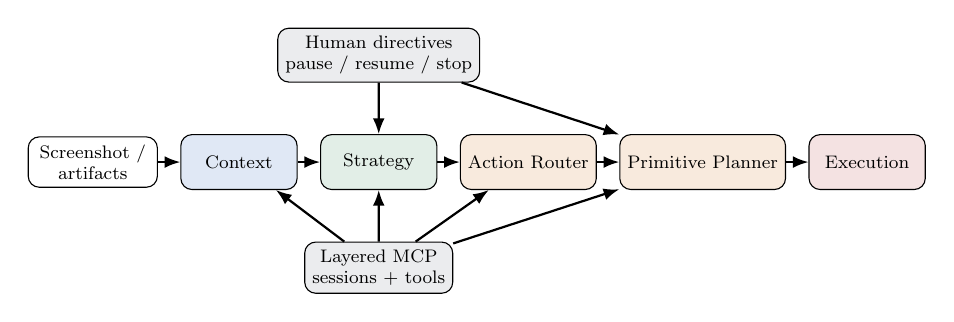
\begin{tikzpicture}[
        scale=0.82,
        transform shape,
        node distance=0.35cm and 0.35cm,
        box/.style={draw, rounded corners, align=center, minimum width=2.0cm, minimum height=0.78cm, font=\footnotesize, fill=white},
        side/.style={draw, rounded corners, align=center, minimum width=2.1cm, minimum height=0.78cm, font=\footnotesize, fill=layergray!12},
        contextbox/.style={draw, rounded corners, align=center, minimum width=1.8cm, minimum height=0.85cm, font=\footnotesize, fill=layerblue!16},
        strategybox/.style={draw, rounded corners, align=center, minimum width=1.8cm, minimum height=0.85cm, font=\footnotesize, fill=layergreen!16},
        actionbox/.style={draw, rounded corners, align=center, minimum width=1.8cm, minimum height=0.85cm, font=\footnotesize, fill=layerorange!16},
        execbox/.style={draw, rounded corners, align=center, minimum width=1.8cm, minimum height=0.85cm, font=\footnotesize, fill=layerred!16},
        arr/.style={-{Latex[length=2mm]}, thick}
    ]
    \node[box] (capture) {Screenshot /\\artifacts};
    \node[contextbox, right=of capture] (context) {Context};
    \node[strategybox, right=of context] (strategy) {Strategy};
    \node[actionbox, right=of strategy] (router) {Action Router};
    \node[actionbox, right=of router] (primitive) {Primitive Planner};
    \node[execbox, right=of primitive] (execute) {Execution};

    \node[side, above=0.8cm of strategy] (human) {Human directives\\pause / resume / stop};
    \node[side, below=0.8cm of strategy] (mcp) {Layered MCP\\sessions + tools};

    \draw[arr] (capture) -- (context);
    \draw[arr] (context) -- (strategy);
    \draw[arr] (strategy) -- (router);
    \draw[arr] (router) -- (primitive);
    \draw[arr] (primitive) -- (execute);
    \draw[arr] (human) -- (strategy);
    \draw[arr] (human) -- (primitive);
    \draw[arr] (mcp) -- (context);
    \draw[arr] (mcp) -- (strategy);
    \draw[arr] (mcp) -- (router);
    \draw[arr] (mcp) -- (primitive);
    \end{tikzpicture}
    \caption{CivStation's runtime philosophy: the live loop is layered, and both human directives and MCP sessions can intervene around the same state transitions.}
    \label{fig:runtime-philosophy}
\end{figure}

\section{Layered Runtime Architecture}

\subsection{From screenshot to execution}

The core runtime path is straightforward to state and deliberately structured to be inspectable: capture a screenshot, update state, refine strategy, route the screenshot to the appropriate primitive, plan an action in normalized coordinates, and finally execute that action on the local machine. Figure~\ref{fig:runtime-philosophy} summarizes the flow.

The \texttt{Context} layer maintains shared state for the rest of the stack. According to the repository documentation, this includes global game state, high-level threats and opportunities, and primitive-local execution history \cite{civstation_repo}. Background workers can update summaries and turn-detection information without blocking the main step loop. This design separates ``what the system knows'' from ``what the system does next.''

The \texttt{Strategy} layer translates free-form human or autonomous guidance into a structured strategy object. Instead of leaving strategic intent as a raw string forever, CivStation represents it as a structured plan with fields such as victory goal, phase, and primitive directives. This is important in a game like Civilization VI because the same screenshot may invite different local actions under different high-level goals. A governor promotion, a research choice, and a diplomacy screen all depend on current strategy, not only current pixels.

The \texttt{Action} layer is itself split into routing and primitive-specific planning. This is one of the system's most important design decisions. The router classifies the screenshot into a primitive. The primitive planner then generates the next executable action for that mode. In the repository snapshot used for this paper, the primitive registry contains 12 routable primitives and 2 human-forced primitives. The routable set covers religion, governors, voting, era selection, unit operations, research selection, city production, culture, diplomacy, combat, policy management, and generic popups. The human-forced set covers war declarations and deal handling. A single registry defines criteria, prompts, priorities, multi-step behavior, and completion conditions for these primitives, which keeps routing, prompting, and extension logic aligned.

Finally, execution is isolated behind normalized coordinates. Models are asked to emit actions in a fixed coordinate range, and the runtime restores those coordinates to the actual monitor or game-window resolution only at the execution boundary. This allows the same action representation to survive across display settings, game-window crops, and Retina/logical-pixel mismatches. In practical terms, the VLM does not need to know the user's absolute screen resolution; it only needs to act within a normalized action space that the runtime can faithfully map back into real coordinates.

\subsection{Human-in-the-loop as a first-class layer}

The \texttt{HitL} layer is not an afterthought. It is explicitly treated as one of the four architectural layers in the README and module documentation \cite{civstation_repo}. The layer provides lifecycle control, command queuing, turn checkpoints, and status broadcasting. Pending directives are prioritized in a deterministic order, with stop requests taking precedence over primitive overrides, pause requests, and strategy changes. This matters because intervention semantics are part of system correctness: a safe stop must not be blocked by a lower-priority strategy change.

The operator-facing implementation includes a FastAPI dashboard, REST endpoints, WebSocket control, and an external relay path for phone-based control through the \texttt{tacticall} controller stack \cite{tacticall_repo}. This turns CivStation into a supervised autonomy system rather than a single-user script. Researchers can observe live traces, developers can interrupt multi-step primitive flows, and remote operators can steer a game session without SSHing into the host machine.

\subsection{MCP as a stable control plane}

MCP's architecture distinguishes hosts, clients, and servers and defines data-layer primitives such as tools, resources, and prompts \cite{mcp_architecture}. CivStation adopts this pattern by wrapping its layered runtime in an MCP server. The current server implementation exposes 29 tools across session management, context, strategy, memory, action, human control, and end-to-end workflow orchestration.

The resulting session model is one of CivStation's most practically useful features. Each session owns its own context, memory, HITL queue and gate state, runtime configuration, adapter overrides, and last captured artifacts. This lets an external client branch, inspect, or replay state without mutating one global process. It also supports per-session adapter swapping, which means the same external contract can be preserved while the internal router, planner, observer, refiner, or executor changes. For a research codebase, this is a strong separation of interface from implementation.

\subsection{Why primitive routing matters}

Primitive decomposition is especially important in Civilization VI because the interface is mode-heavy. Research choice, policy selection, governor assignment, diplomacy, and city production all impose different action grammars and different failure modes. A single large prompt can in principle handle all of them, but it becomes harder to debug, harder to localize errors, and harder to adapt under human intervention. CivStation's primitive registry acts as a task router and a systems contract at the same time: each primitive defines routing criteria, prompting context, multi-step behavior, and completion logic in one place. That makes the decomposition operational rather than merely conceptual.

\begin{table}[t]
\centering
\caption{Repository snapshot summarized from the codebase inspected for this paper.}
\label{tab:project-snapshot}
\begin{tabular}{p{2.0cm} p{5.0cm}}
\toprule
\textbf{Item} & \textbf{Value} \\
\midrule
Project name & CivStation (package name still \texttt{civStation}; module name \texttt{computer\_use\_test}) \\
Source layout & 123 Python source files; 48 files under \texttt{tests/} \\
Primitives & 12 routable primitives, 2 HitL-only primitives \\
MCP surface & 29 tools spanning session, context, strategy, memory, action, HitL, and workflow \\
Live control & Local dashboard, REST, WebSocket, remote phone-controller path \\
Evaluation & Legacy Civ6 evaluator plus bounding-box-based evaluator with external agent runners \\
CI & GitHub Actions linting plus tests on Python 3.12 and 3.13 \\
Local verification & 96 targeted tests passed in the repository's \texttt{.venv}, including turn executor, HitL, parser, MCP, and bbox evaluation tests \\
\bottomrule
\end{tabular}
\end{table}

To obtain a minimal real-provider comparison, we also generated a small synthetic UI benchmark with three cases (confirm-button click, escape-to-dismiss, and drag action) and ran multiple frontier models through the same bbox evaluator. The result is not a benchmark claim about general capability, but it is informative about variability across models and action types. In this synthetic setting, Claude Sonnet 4 solved two of three tasks, whereas the two GPT variants used in the study did not solve any of the three tasks. The main failure modes were keypress generation and drag/click mismatches, which suggests that even very small benchmark suites can reveal materially different action priors across model families.

\begin{table}[t]
\centering
\caption{Preliminary cross-model results on the synthetic 3-case UI benchmark.}
\label{tab:cross-model}
\begin{tabular}{lcc}
\toprule
\textbf{Model} & \textbf{Strict success} & \textbf{Avg. step acc.} \\
\midrule
GPT-4o-mini & 0.000 & 0.000 \\
GPT-4o & 0.000 & 0.000 \\
Claude Sonnet 4 & 0.667 & 0.667 \\
\bottomrule
\end{tabular}
\end{table}

\section{Control Interfaces and Evaluation Stack}

\subsection{Operator interfaces}

Table~\ref{tab:project-snapshot} highlights that CivStation's control philosophy is reflected in its software surface. A user can run the live agent with a local dashboard, issue REST calls, send WebSocket messages, or bridge control through the remote phone interface. The live agent therefore has multiple ingress points for intervention and status inspection.

This is more than convenience. In long-horizon gameplay, the ability to stop or redirect execution is a core systems property. A planner can be locally correct and globally unhelpful. For example, a primitive may select a technically legal action while ignoring a higher-level strategic shift requested by a human operator. CivStation's interface design makes those strategy changes and primitive overrides part of the supported workflow rather than special-case debugging behavior.

\subsection{Static evaluators}

The repository also contains a static evaluation subsystem. The older evaluator focuses on Civilization VI primitive selection and action generation with coordinate tolerance, while the newer \texttt{bbox\_eval} pipeline reframes action correctness in terms of bounding-box targets rather than exact pixel matches. This newer evaluator supports multiple acceptable action sequences per case, richer sequence-level metrics, and external agent integration through a subprocess protocol. Those choices make the evaluation stack more suitable for comparing imperfect but still acceptable UI actions.

This distinction matters in practice. Exact-pixel evaluation is often too brittle for computer-use agents because multiple click locations or action orders may be semantically equivalent. Bounding boxes and multiple ground-truth sets improve tolerance without giving up structure. CivStation therefore treats evaluation not as one score-producing script, but as an extensible framework with reusable schemas, agent runners, and dataset loaders.

\subsection{Current validation status}

Although CivStation is still alpha-stage software, the repository already supports targeted validation of several key interfaces. In the environment used for this paper, the repository's local virtual environment passed 96 targeted tests across the turn executor, human-in-the-loop command queue, state bridge, parser logic, layered MCP server, and bounding-box scorer. The repository also contains GitHub Actions configuration for linting and tests on Python 3.12 and 3.13. This is not a substitute for a full empirical benchmark on live gameplay, but it does provide evidence that the system's main software abstractions are exercised by automated tests rather than being documented only informally.

We also ran a small end-to-end sanity check on the repository's sample bounding-box dataset. The same evaluation pipeline cleanly separates a deliberately mismatched mock policy from a reference policy that clicks bbox centers and reproduces the expected action sequence. Table~\ref{tab:sanity-eval} reports these results. They should be read as software-validation checks rather than competitive agent benchmarks, but they provide a minimal quantitative anchor for the evaluator itself.

\begin{table}[t]
\centering
\caption{Sanity-check results on the sample bbox evaluation dataset (3 cases).}
\label{tab:sanity-eval}
\begin{tabular}{lcc}
\toprule
\textbf{Runner} & \textbf{Strict success} & \textbf{Avg. step acc.} \\
\midrule
MockAgentRunner & 0.00 & 0.00 \\
Perfect reference runner & 1.00 & 1.00 \\
\bottomrule
\end{tabular}
\end{table}

\begin{table*}[t]
\centering
\caption{Positioning CivStation relative to representative computer-use systems.}
\label{tab:related-systems}
\scriptsize
\begin{tabular}{p{1.55cm} p{1.55cm} p{1.8cm} p{2.0cm} p{3.7cm}}
\toprule
\textbf{System} & \textbf{Domain} & \textbf{Human steering} & \textbf{Control plane} & \textbf{Action eval} \\
\midrule
Anthropic computer use \cite{anthropic_computer_use} & General desktop interaction & Tool-loop dependent; implementation left to developers & API tool interface & No repository-level benchmark framework exposed in the docs page \\
Browser Use \cite{browser_use} & Browser automation & Possible through custom tooling, but not the central abstraction & Library, CLI, cloud, MCP/custom tool integrations & External benchmark repo; not focused on turn-based game evaluation \\
OpenHands \cite{openhands_docs, openhands_repo} & AI-driven development & Yes, through CLI/GUI workflows and platform controls & SDK, CLI, GUI, integrations, MCP support in docs & Evaluation infrastructure exists, but not specialized for visual game-action scoring \\
OSWorld \cite{osworld_project} & Benchmarking multimodal computer-use agents & Not the main goal & Benchmark environment and project tooling & Yes, as a benchmark for real computer tasks \\
Voyager \cite{voyager} & Open-ended Minecraft agent & Limited operator-facing control emphasis & Research code and skill library paradigm & Focused on embodied learning, not UI-action evaluation \\
\textbf{CivStation} \cite{civstation_repo} & Civilization VI computer use & \textbf{Yes; dashboard, REST, WebSocket, remote controller} & \textbf{Layered MCP server plus local control surfaces} & \textbf{Yes; legacy Civ6 evaluator and bbox-based evaluator in one repo} \\
\bottomrule
\end{tabular}
\end{table*}

\section{Image Preprocessing, Latency, and VLM Action Reliability}

One of the practical novelties of CivStation is that it exposes image-preprocessing and transport decisions as explicit experimental knobs rather than hiding them behind a single screenshot function. The default screen utilities downscale images to a long edge of 1280 pixels and use JPEG quality 80, with the architecture notes estimating that this cuts image-token load by roughly 75\% while keeping game text readable. On top of that default, the repository provides an \texttt{ImagePipelineConfig} abstraction and reusable UI filters, color policies, and simulated transport encodings for targeted experiments.

This matters because VLM action quality is coupled to payload design. The codebase includes presets for routers, planners, context updates, turn detection, and harder planner regimes such as policy and city-production screens. It also includes a rough benchmarking harness for policy-screen action extraction under different prompt lengths, normalization ranges, image sizes, background treatments, and preprocessing pipelines. In the saved report checked into the repository, raw images averaged 6.179 seconds per inference on a single benchmark screenshot, while compressed and compressed-downscaled variants averaged 3.609 and 3.667 seconds respectively. The same report showed smaller but measurable effects from prompt length and coordinate range, and much smaller average effects from background color padding.

\begin{table}[t]
\centering
\caption{Exploratory latency summary from the saved rough policy-extraction report using \texttt{gemini-3-flash-preview}.}
\label{tab:latency-tradeoffs}
\begin{tabular}{lc}
\toprule
\textbf{Condition} & \textbf{Mean latency (s)} \\
\midrule
Range 250 & 4.167 \\
Range 500 & 4.392 \\
Range 1000 & 4.579 \\
Concise prompt & 4.249 \\
Long prompt & 4.510 \\
Compressed image & 3.609 \\
Compressed + downscale restore & 3.667 \\
Downscale restore & 4.063 \\
Raw image & 6.179 \\
\bottomrule
\end{tabular}
\end{table}

Table~\ref{tab:latency-tradeoffs} should be interpreted carefully. It is an exploratory artifact, not a full benchmark section. Still, it is useful because it captures the systems reality that VLM action is strongly affected by transport and preprocessing choices. In particular, the rough report suggests that image size mode had a much larger impact on latency than background padding, and that reducing the coordinate normalization range from 1000 to 250 yielded a modest average speedup. CivStation's benchmarking code also defines a quality gate that marks a preprocessing variant as acceptable only if its strict-success rate and average step accuracy stay within five percentage points of a baseline. This makes the trade-off explicit: a faster screenshot pipeline is only interesting if the action policy does not collapse.

We also ran a smaller real-provider trade-off sweep with GPT-4o-mini on synthetic benchmark assets. In that run, the fastest measured configuration used a 500-point coordinate range, a long prompt, and a downscaled image with contrast-enhanced JPEG-like preprocessing, reaching 1.791 seconds average latency. The best quality row on the tiny three-case synthetic dataset reached 0.333 strict-success rate and 0.333 average step accuracy at roughly 3.014 seconds. Although these numbers are far from sufficient for a headline result, they provide a concrete example of the paper's central claim: latency and action quality move together, and the point of the infrastructure is to make that trade-off measurable rather than anecdotal.

The repository's saved rough reports also reflect a practical development pattern: exploratory trade-off work was centered on Gemini Flash because it was the most convenient model family for repeated image-variant sweeps during development. However, the fresh paper-preparation run reported here could not reproduce a live Gemini comparison because the configured Gemini API key had expired. We therefore treat ``Gemini Flash felt least error-prone during iterative development'' as a developer-side empirical impression rather than as a finalized benchmark claim.

\paragraph{Where VLM action works well.}
The design of CivStation reflects an empirical bias toward UI states with clear affordances and bounded action grammars. Research-choice dialogs, modal popups, policy slots, governor screens, and other discrete interfaces are well matched to primitive routing and normalized coordinates. In these settings, the action space is small enough that prompt specialization and operator overrides are effective.

\paragraph{Where VLM action remains brittle.}
The codebase also makes clear what is hard. Policy management, city production, and other multi-step interfaces receive dedicated multi-step logic and higher-quality image presets, which signals that dense UI, drag-and-drop behavior, and stateful confirmation flows are failure-prone regimes. Raw full-resolution screenshots are slower, which increases the practical cost of simply throwing more pixels at the problem. More generally, local action quality does not solve strategic coherence by itself; it must still be conditioned on longer-horizon state and human guidance.

\section{Research Trends and CivStation's Contribution Gap}

Current computer-use research is moving along at least three fronts. First, proprietary frontier systems are turning computer use into a general tool interface, as seen in Anthropic's computer-use tooling and OpenAI's Computer-Using Agent announcement \cite{anthropic_computer_use, openai_cua}. Second, open-source operational stacks are making these capabilities easier to script and deploy, particularly for browsers and software engineering workflows, as exemplified by Browser Use and OpenHands \cite{browser_use, openhands_docs, openhands_repo}. Third, the field is rapidly building benchmark ecosystems, with projects such as OSWorld and OSUniverse emphasizing real computer environments, multimodal interfaces, and automated validation \cite{osworld_project, osuniverse}.

These trends are valuable, but they still leave a gap for strategy-heavy, persistent, long-horizon environments. OSUniverse explicitly targets short- and medium-term GUI tasks and automated validation, which is useful for measuring progress on immediate interaction competence \cite{osuniverse}. Browser-use stacks emphasize websites. Software-agent stacks emphasize coding tasks. Embodied-game work such as Voyager emphasizes open-ended skill accumulation \cite{voyager}. What remains underexplored is a benchmark substrate where strategic planning, persistent state, operator steerability, and action-level validation all coexist in one reproducible environment.

That is the niche CivStation is trying to define. Its novelty is not that Civilization VI is a game and games are hard. The novelty is that a turn-based strategy game can become a useful systems laboratory for computer use. The environment provides delayed consequences, structured turns, interpretable micro-actions, and an interface rich enough to stress perception, planning, and intervention. CivStation contributes a software architecture that makes those properties measurable rather than anecdotal.

\section{Civilization VI as a Long-Horizon Benchmark Substrate}

Civilization VI has several properties that make it more than an application target. First, it is persistent: a locally correct action can still be globally poor many turns later. Second, it mixes macro-strategy and micro-execution. A good system must decide what to optimize, then navigate the relevant interface state correctly. Third, the game has stable rules and recognizable turn boundaries, which makes human-versus-agent comparison tractable. Fourth, the interface contains a range of action types, from direct clicks to drags, confirmations, dialog handling, and hierarchical menus. These properties make the domain a plausible bridge between one-step GUI interaction and genuinely long-horizon task evaluation.

This benchmark perspective opens several research directions. One is dynamic LLM benchmarking: because strategy quality can change materially as models improve, the same CivStation task suite could be rerun across model families and over time, with the strategy layer acting as a natural place to observe improvement. Another is human-versus-agent long-horizon comparison. Unlike many opaque desktop tasks, Civilization VI provides a domain in which human strategic play is meaningful, reproducible, and not reducible to a single click sequence. A third is agent-versus-agent evaluation, where different planners or model stacks can be compared under the same persistent state and intervention budget.

Crucially, the benchmark modes that matter most in this domain are live rather than static: human-versus-Civ6-agent play, Civ6-agent-versus-Civ6-agent play, and HITL-supervised Civ6-agent versus fully autonomous Civ6-agent play. Static screenshot datasets remain useful as auxiliary tools, but they do not capture persistent strategic drift, interruption risk, or the full tempo of online play.

The idea generalizes beyond a single game. If VLM-driven computer use becomes robust enough in one turn-based game, the same layered design can be ported to other visual task domains with structured rules. In that sense, CivStation is valuable even if Civilization VI remains only the first fully supported environment. The broader contribution is a path toward long-horizon game-grounded computer-use benchmarks that sit between browser automation and open-world embodied agents.

\section{Operational Safety, Limitations, and Future Work}

Computer-use systems can act on the user's machine, which creates obvious misuse and safety concerns \cite{anthropic_computer_use}. CivStation partially addresses this by giving operators multiple ways to interrupt execution, by separating strategy changes from lower-level actions, and by treating human discussion and directive channels as supported features rather than emergency patches. The system's architecture does not eliminate misuse risk, but it does make trust boundaries more explicit than an opaque loop would.

Several limitations remain. First, the project still lacks a full public benchmark section with live-agent numbers against strong baselines. Second, although the repository includes exploratory latency reports and a quality-benchmark harness, it does not yet include a complete checked-in accuracy-speed Pareto study with real model calls across a representative dataset. Third, the current primitive inventory is hand-authored for Civilization VI, which means portability still depends on substantial domain work. Fourth, the codebase is in a naming transition: the public name is CivStation, but the package and module names remain \texttt{civStation} and \texttt{computer\_use\_test}. Fifth, the local environment used to prepare this paper did not include a LaTeX toolchain, so PDF compilation could not be completed here.

There are also limitations specific to online dynamic experiments. Civilization VI is not a headless benchmark environment in the same sense as a browser task suite. To run an end-to-end live experiment, a human typically has to launch the game, maintain a valid session, and often supervise progress because the model can stall, drift, or get interrupted by modal events. This makes large repeated studies operationally expensive. It also means that online evaluation can fail for reasons that are only partly about the policy itself, including slow inference, broken session state, or interruption in the middle of a multi-step action sequence.

The project also highlights a verification bottleneck. Once a computer-use action is executed, the system still has to decide whether the action actually succeeded and whether to trigger a fallback or recovery path. CivStation contains explicit semantic verification and fallback logic for this reason, but that verification is itself often delegated back to VLM perception. In other words, the controller and the verifier can share the same visual weaknesses. This creates a practical ceiling on how reliable purely vision-driven fallback logic can be today.

These limitations naturally define the next stage of work. Future experiments should quantify when VLM action benefits from higher-resolution inputs and when it merely adds cost; compare fast and high-quality image presets on real datasets; study human intervention frequency and usefulness over long horizons; and test dynamic strategy benchmarking across multiple LLMs. A particularly attractive direction is a hybrid architecture in which VLMs specialize in visual understanding and scene grounding, while faster language or action models handle micro-actions once the state is grounded. That hybrid could reduce the practical tension between visual competence and action latency. It may also reduce error compounding: if visual grounding itself is another vision problem, stacking multiple vision-heavy stages can amplify rather than reduce failure.

Longer-term work should explore agent-agent matchups, human-agent performance comparison under shared tasks, broader cross-game transfer, and automatic primitive discovery rather than hand-authored routing taxonomies. Another promising direction is to train game- or application-specific VLA-style components that can execute native micro-actions reliably inside one target environment, while keeping the higher-level strategic layer open to rapidly improving LLMs. Under that division of labor, CivStation would evolve from a domain stack into a general long-horizon benchmark framework for visual interactive tasks.

\section{Reproducibility and Usage}

From a submission perspective, CivStation aligns well with the reproducibility expectations emphasized by recent NeurIPS and ICLR calls for papers, which explicitly highlight paper checklists, appendices, code availability, ethics, and responsible use of LLMs \cite{neurips_cfp, iclr_cfp}. The repository is public, the architecture is documented at multiple levels, and the MCP surface provides a stable external interface for reproducing or scripting workflows. The evaluation subsystem also lowers the cost of reproducing action-level checks without rerunning live gameplay every time.

The system is already usable in three distinct modes. First, it can run as a live computer-use agent through the turn runner and dashboard. Second, it can be exposed as a layered MCP server for external orchestration. Third, its evaluation modules can be run independently for static screenshot benchmarking. The appendix includes a minimal usage sketch for these workflows so that the paper does not treat CivStation as a black-box artifact.

\section{Conclusion}

CivStation is a systems contribution for researchers and developers who need more than a one-shot game bot. Its central claim is architectural: computer-use agents for long-horizon visual environments benefit from explicit separation between context, strategy, action, and human intervention. Around that claim, the repository packages a practical stack: a primitive-routed live runtime, a layered MCP server with session isolation and adapter swapping, multiple operator control surfaces, and a reusable action-level evaluation subsystem.

For the current state of the project, that is the right unit of contribution. CivStation does not yet claim to solve Civilization VI autonomously at scale. Instead, it offers something the field still needs: a controllable and inspectable substrate for studying long-horizon computer use under persistent state, strategic choice, and human supervision. If that substrate proves reusable, then its value extends beyond a single game. It becomes a path toward dynamic LLM benchmarking, human-versus-agent comparison, and eventually game-grounded long-horizon testbeds for VLM-based computer-use research more broadly.

\appendix

\section{Minimal Usage}

\paragraph{Live agent.}
\begin{quote}
\ttfamily
python -m computer\_use\_test.agent.turn\_runner --provider claude --turns 100 --strategy "Focus on science victory" --status-ui --wait-for-start --status-port 8765
\end{quote}

\paragraph{Layered MCP server.}
\begin{quote}
\ttfamily
python -m computer\_use\_test.mcp.server
\end{quote}

\paragraph{Static bbox evaluator.}
\begin{quote}
\scriptsize\ttfamily
python -m computer\_use\_test.evaluation.evaluator.action\_eval.bbox\_eval\\
--dataset path/to/dataset.jsonl\\
--provider claude
\end{quote}

\paragraph{Paper artifacts.}
\begin{quote}
\ttfamily
python docs/paper/scripts/generate\_paper\_artifacts.py
\end{quote}

\paragraph{Cross-model benchmark.}
\begin{quote}
\ttfamily
python docs/paper/scripts/run\_paper\_cross\_model\_benchmark.py
\end{quote}

\paragraph{Trade-off benchmark.}
\begin{quote}
\ttfamily
python docs/paper/scripts/run\_paper\_gemini\_tradeoff.py
\end{quote}

\paragraph{Typical research workflow.}
In practice, a researcher can use CivStation in three passes: first, run the live agent with dashboard supervision; second, expose or script the same workflow through MCP; third, move specific UI states into the static evaluator for reproducible action-level analysis. This is the sense in which CivStation is intended to function both as an agent stack and as a benchmark substrate.

\section{Architecture Details}

\paragraph{Layer responsibilities.}
The \texttt{Context} layer tracks game observations and long-horizon notes. The \texttt{Strategy} layer translates free-form intent into structured strategic state. The \texttt{Action} layer splits into routing and primitive planning. The \texttt{HitL} layer controls pause, resume, stop, overrides, and discussions. This partition is important because the failure modes are different at each level.

\paragraph{Verification and fallback.}
CivStation does not assume that a generated action succeeded just because it was executed. Multi-step primitives include semantic verification and staged fallback logic, especially for dense or stateful screens such as policy management, religion, and research entry. This is a major practical requirement in computer-use systems, since a failed click, a missed drag, or a modal interruption can invalidate an entire chain of later actions.

\paragraph{Hybrid direction.}
The repository already contains explicit TODO notes toward hybrid context extraction, where native game data and VLM-based perception would be combined. This points toward a broader future architecture in which fast action models, native-app-specific VLAs, or symbolic/native instrumentation cooperate with VLM-based visual understanding rather than replacing it.

\section{Synthetic Benchmark Assets}

The paper bundle includes a synthetic UI benchmark because the checked-in Civ bbox fixtures do not include their screenshot files. The synthetic set is only a fallback artifact for paper preparation. It is not the intended final benchmark substrate. The real benchmark vision for CivStation remains live Civilization VI play. The synthetic set has three cases:
\begin{itemize}[leftmargin=*]
    \item a confirm-button click
    \item an escape-to-dismiss dialog
    \item a drag from a center target to an upper-left target
\end{itemize}
These cases are intentionally simple. They are not meant to substitute for a real Civilization VI benchmark. Their role is to provide a reproducible sanity harness for model- and preprocessing-level comparisons when real game screenshots are unavailable.

\section{Online Experiment Constraints}

Running a live Civilization VI experiment is operationally different from scoring an offline browser benchmark. A human usually has to start the game, maintain window focus, and monitor session health. Slow inference can make the system miss the tempo of interaction. Interruptions, popups, or state drift can break a run even when the high-level policy is reasonable. For this reason, many of the current results in the paper should be read as \emph{empirical systems observations} rather than as definitive benchmark statements. The benchmark substrate is promising, but large-scale online experimentation remains an engineering bottleneck in its own right.


\bibliographystyle{IEEEtran}
\bibliography{ref}

\end{document}
